%% Submissions for peer-review must enable line-numbering
%% using the lineno option in the \documentclass command.
%%
%% Preprints and camera-ready submissions do not need
%% line numbers, and should have this option removed.
%%
%% Please note that the line numbering option requires
%% version 1.1 or newer of the wlpeerj.cls file, and
%% the corresponding author info requires v1.2

\documentclass[fleqn,10pt,lineno]{wlpeerj} % for journal submissions

% ZNK -- Adding headers for pandoc

\setlength{\emergencystretch}{3em}
\providecommand{\tightlist}{
\setlength{\itemsep}{0pt}\setlength{\parskip}{0pt}}
\usepackage{lipsum}
\usepackage[unicode=true]{hyperref}
\usepackage{longtable}



\usepackage{lipsum}

\title{Juvenile Salmon Migration Dynamics in the Discovery Islands and
Johnstone Strait in 2018}

\author[1]{Brett T. Johnson}

\corrauthor[1]{Brett T. Johnson}{\href{mailto:brett.johnson@hakai.org}{\nolinkurl{brett.johnson@hakai.org}}}
\author[]{Julian C.L. Gan}

\author[2, 3]{Brian P.V. Hunt}


\affil[1]{Hakai Institute Quadra Island Ecological Observatory, Heriot Bay, BC
V0P1H0}
\affil[2]{UBC EOS, IOF}


%
% \author[1]{First Author}
% \author[2]{Second Author}
% \affil[1]{Address of first author}
% \affil[2]{Address of second author}
% \corrauthor[1]{First Author}{f.author@email.com}

% 


\begin{abstract}
The majority of out-migrating juvenile Fraser River salmon pass
northwest through the Strait of Georgia, the Discovery Islands, and
Johnstone Strait. The Discovery Islands to Johnstone Strait leg of the
migration is a region of poor survival for juvenile salmon relative to
the Strait of Georgia. The Hakai Institute Juvenile Salmon Program has
been monitoring key components of this migration since 2015 to better
understand drivers of early marine survival. Here we present key aspects
of the 2018 migration in comparison to averages from the 2015---2018
study period, which we use to define `normal'. In 2018 sockeye, pink,
and chum all migrated earlier than normal. The median capture date was
May 23rd for sockeye, five days earlier than normal, and June 12 for
pink and chum which is five days earlier for pink and three days earlier
than normal for chum. Sea lice prevalence was lower than normal for
sockeye, pink, and chum. Notably there were no \emph{Lepeoptheirus
salmonis} sea lice observed in Johnstone Strait in 2018. Sockeye were
longer than normal in 2018 whereas pink and chum were smaller than
normal. Sea surface temperature in May and June was the warmest on
record in the study period (2015---2018). Pink salmon dominated the
catch in 2018, followed by chum and then sockeye.
% Dummy abstract text. Dummy abstract text. Dummy abstract text. Dummy abstract text. Dummy abstract text. Dummy abstract text. Dummy abstract text. Dummy abstract text. Dummy abstract text. Dummy abstract text. Dummy abstract text.
\end{abstract}

\usepackage{amsthm}
\newtheorem{theorem}{Theorem}[section]
\newtheorem{lemma}{Lemma}[section]
\theoremstyle{definition}
\newtheorem{definition}{Definition}[section]
\newtheorem{corollary}{Corollary}[section]
\newtheorem{proposition}{Proposition}[section]
\theoremstyle{definition}
\newtheorem{example}{Example}[section]
\theoremstyle{definition}
\newtheorem{exercise}{Exercise}[section]
\theoremstyle{remark}
\newtheorem*{remark}{Remark}
\newtheorem*{solution}{Solution}
\begin{document}

\flushbottom
\maketitle
\thispagestyle{empty}

\section*{Introduction}\label{introduction}
\addcontentsline{toc}{section}{Introduction}

Pacific salmon (\emph{Oncorhynchus} spp.) traverse a number of aquatic
landscapes during different phases of their lifecyle to reach a habitat
which ultimately offers some reward. While undergoing these migrations,
salmon are subjected to risks associated with each new environemnt they
encounter. The risks and associated mortality from the sum of these
migrations can be understood in aggregate by quantifying the
productivity (recruits per spawner) of a certain stock. Salmon are an
excellent indicator species beacuse they act as an integrator of
terrestrial, lacustrine, fluvial, estuarine, nearshore marine, and
high-seas conditions. A problem in any one of these environments will be
reflected in the productivity of salmon stocks. To better manage and
predict the producitivty of salmon stocks we need estimates of mortality
and an understanding of the factors driving mortality in each landscape
that salmon traverse. The early marine environment is one which
estimates of mortality and it's drivers, is lacking. Juvenile salmon are
particularly vulnerable during the early marine phase of their life
history because they are undergoing physiological adaptations to a
saline environment.

The Hakai Institute Juvenile Salmon Program has been monitoring juvenile
salmon migrations in the Discovery Islands and Johnstone Strait (Figure
\ref{fig:map}) 2015 in an effort to understand what factors may be
influencing early marine survival of sockeye, pink, and chum (Hunt et
al. 2018). The effects of pathogens, parasites, predators, and the
impacts of climate change on food web dynamics may be amplified during
this stressful transition period and are the primary aspects of the
salmon migration we are monitoring and reporting on here.

\begin{figure}

\includegraphics[width=450pt]{map} \hfill{}

\caption{Sampling locations in 2018}\label{fig:map}
\end{figure}

\section*{Methods}\label{methods}
\addcontentsline{toc}{section}{Methods}

See Hunt et al. (2018) for a detailed description of field and lab
methods. Briefly, we collect juvenile salmon weekly from the Discovery
Islands and Johnstone Strait during their northward migration from the
Strait of Georgia to Queen Charlotte Strait near northern Vancouver
Island, British Columbia. Sampling is conducted from May to July each
year since 2015 using purse seine nets (bunt: 27 m x 9 m with 13 mm
mesh; tow: 46 m x 9 m with 76 mm mesh). We sample in nearshore marine
habitats with depth \textgreater{} 10 m and effectively sample sockeye
(\emph{Oncorhynchus nerka}), pink (\emph{O. gorbuscha}), chum (\emph{O.
keta}) and invidentally capture coho (\emph{O. kisutch}), chinook
(\emph{O. tshawytschya}) and pacific herring (\emph{Clupea pallasii})

\section*{Results}\label{results}
\addcontentsline{toc}{section}{Results}

\subsection{Migration Timing}\label{migration-timing}

\section*{\texorpdfstring{Some \LaTeX{}
Examples}{Some  Examples}}\label{some-examples}
\addcontentsline{toc}{section}{Some \LaTeX{} Examples}

Use section and subsection commands to organize your document. \LaTeX{}
handles all the formatting and numbering automatically. Use ref and
label commands for cross-references.

\subsection*{Figures and Tables}\label{figures-and-tables}
\addcontentsline{toc}{subsection}{Figures and Tables}

Use the table and tabular commands for basic tables --- see Table
\ref{tab:widgets}, for example. You can upload a figure (JPEG, PNG or
PDF) using the project menu. To include it in your document, use the
includegraphics command as in the code for Figure \ref{fig:view} below.

Standard \LaTeX references will work as well (e.g.~Fig. \ref{fig:view}).

\begin{figure}
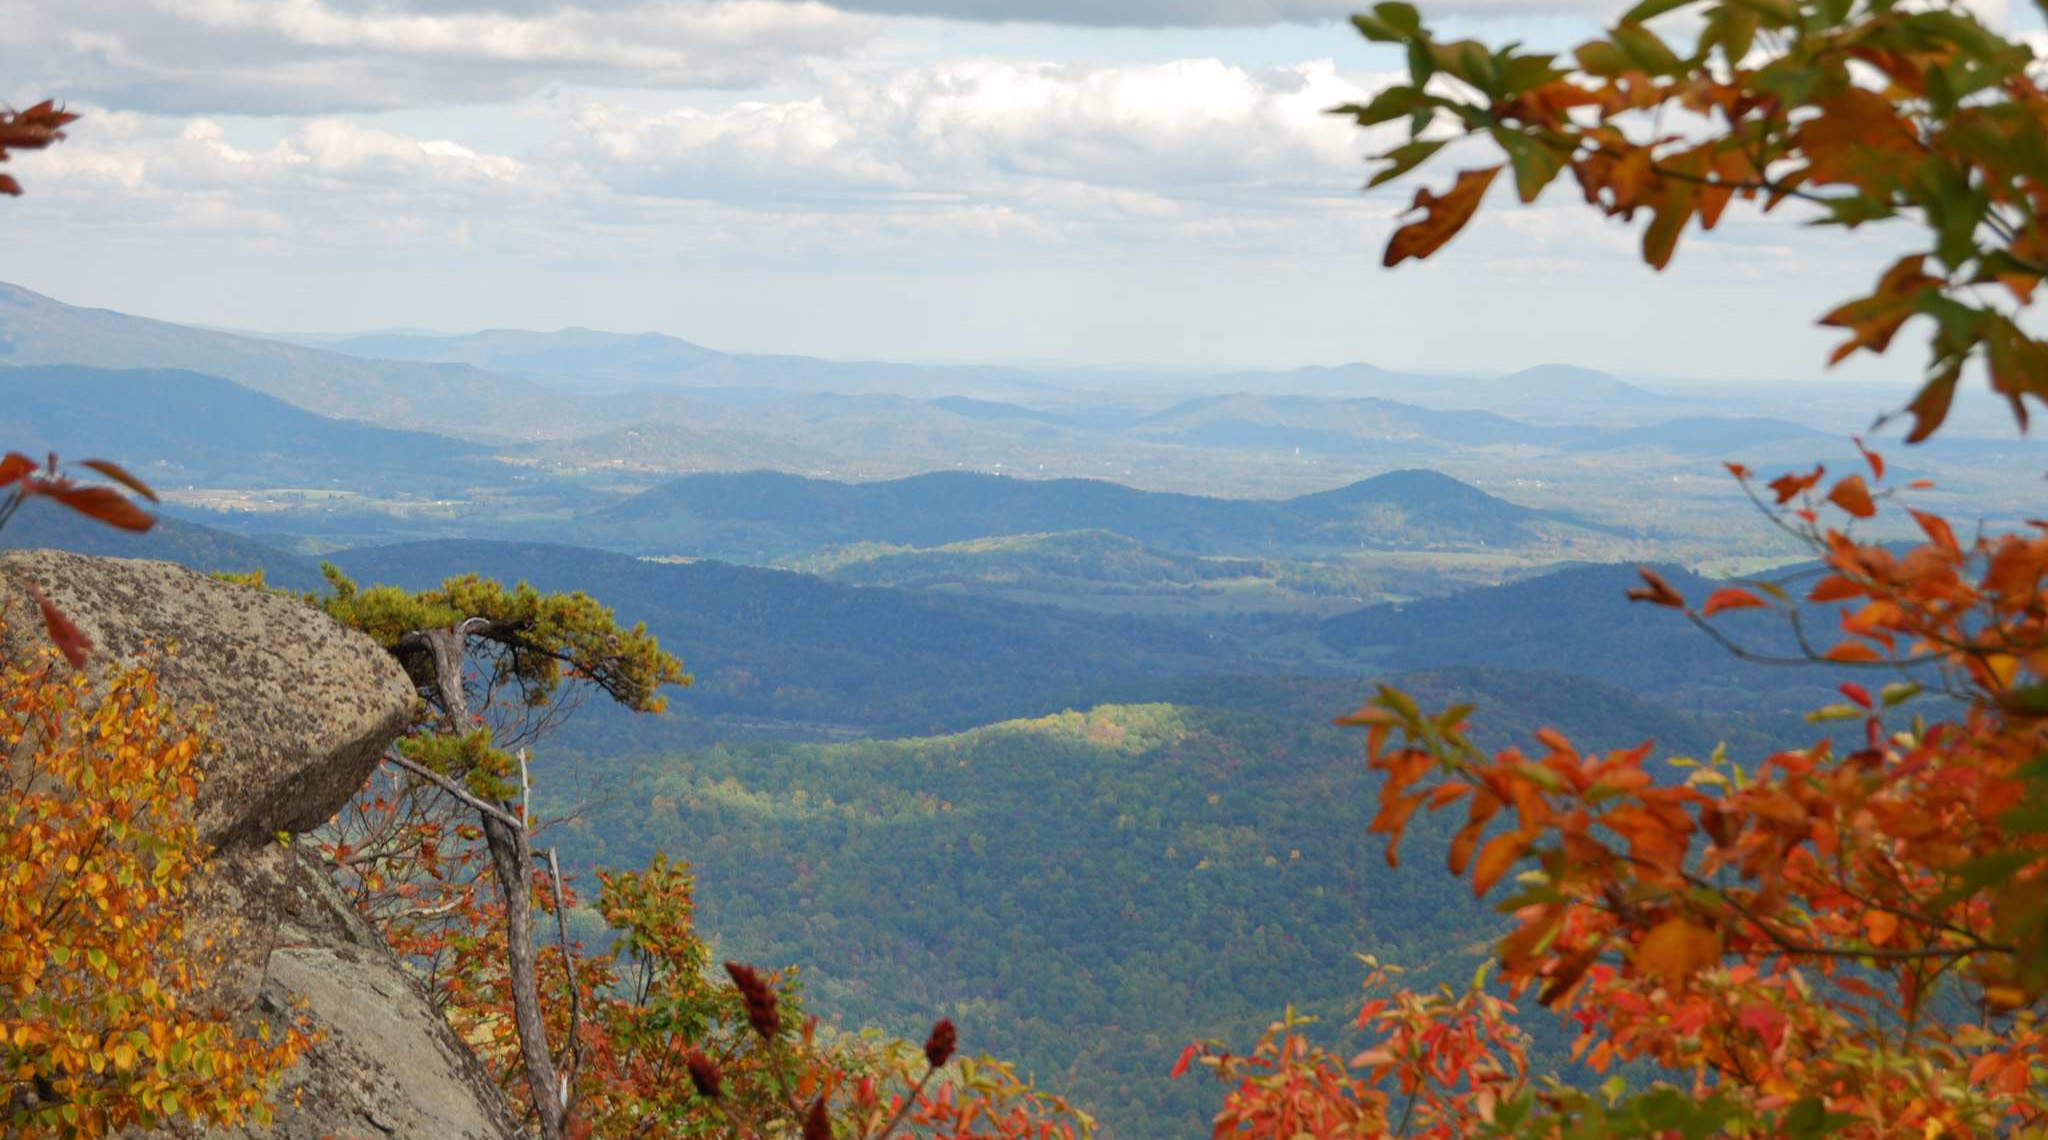
\includegraphics[width=1\linewidth]{view} \caption{An example image.}\label{fig:view}
\end{figure}

\begin{longtable}[]{@{}lr@{}}
\caption{\label{tab:widgets} An Example Table.}\tabularnewline
\toprule
Item & Quantity\tabularnewline
\midrule
\endfirsthead
\toprule
Item & Quantity\tabularnewline
\midrule
\endhead
Widgets & 42\tabularnewline
Gadgets & 13\tabularnewline
\bottomrule
\end{longtable}

\subsection*{Citations}\label{citations}
\addcontentsline{toc}{subsection}{Citations}

LaTeX formats citations and references automatically using the
bibliography records in your .bib file, which you can edit via the
project menu. Use the cite command for an inline citation, like
Figueredo and Wolf (2009), and the citep command for a citation in
parentheses (Figueredo and Wolf 2009).

\subsection*{Mathematics}\label{mathematics}
\addcontentsline{toc}{subsection}{Mathematics}

\LaTeX{} is great at typesetting mathematics. Let
\(X_1, X_2, \ldots, X_n\) be a sequence of independent and identically
distributed random variables with \(\text{E}[X_i] = \mu\) and
\(\text{Var}[X_i] = \sigma^2 < \infty\), and let
\[S_n = \frac{X_1 + X_2 + \cdots + X_n}{n}
      = \frac{1}{n}\sum_{i}^{n} X_i\] denote their mean. Then as \(n\)
approaches infinity, the random variables \(\sqrt{n}(S_n - \mu)\)
converge in distribution to a normal \(\mathcal{N}(0, \sigma^2)\).

\subsection*{Lists}\label{lists}
\addcontentsline{toc}{subsection}{Lists}

You can make lists with automatic numbering \dots

\begin{enumerate}
\def\labelenumi{\arabic{enumi}.}
\tightlist
\item
  Like this,
\item
  and like this.
\end{enumerate}

or bullet points\ldots{}

\begin{itemize}
\tightlist
\item
  Like this,
\item
  and like this.
\end{itemize}

or with descriptions\ldots{}

\begin{itemize}
\tightlist
\item
  \textbf{Word} Definition
\item
  \textbf{Concept} Explanation
\item
  \textbf{Idea} Text
\end{itemize}

We hope you find write\LaTeX~useful for your PeerJ submission, and
please let us know if you have any feedback. Further examples with dummy
text are included in the following pages.

\section*{Methods}\label{methods-1}
\addcontentsline{toc}{section}{Methods}

\lipsum[4] 

\begin{equation}
\cos^3 \theta =\frac{1}{4}\cos\theta+\frac{3}{4}\cos 3\theta
\label{eq:refname2}
\end{equation}

\lipsum[5] 

\subsection*{Subsection}\label{subsection}
\addcontentsline{toc}{subsection}{Subsection}

\lipsum[6] 

\paragraph{Paragraph}

\lipsum[7]  \paragraph{Paragraph} \lipsum[8] 

\subsection*{Subsection}\label{subsection-1}
\addcontentsline{toc}{subsection}{Subsection}

\lipsum[9] 

\begin{figure}
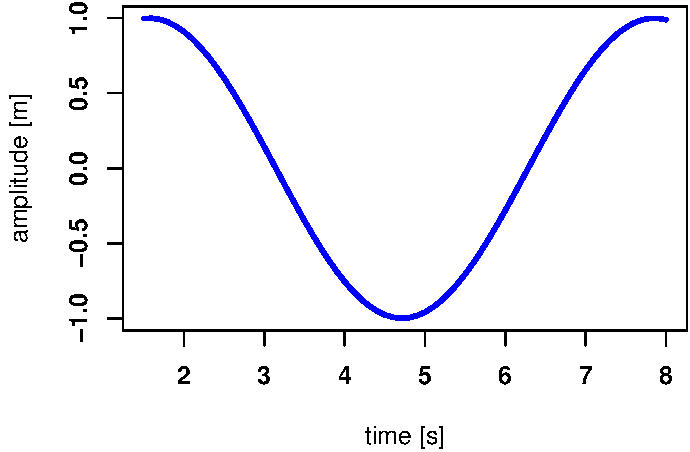
\includegraphics[width=1\linewidth]{peer_j_migration_dynamics_files/figure-latex/results-1} \caption{In-text Picture}\label{fig:results}
\end{figure}

Reference to Figure \ref{fig:results}.

\section*{Results and Discussion}\label{results-and-discussion}
\addcontentsline{toc}{section}{Results and Discussion}

\lipsum[10] 

\subsection*{Subsection}\label{subsection-2}
\addcontentsline{toc}{subsection}{Subsection}

\lipsum[11] 

\subsubsection*{Subsubsection}\label{subsubsection}
\addcontentsline{toc}{subsubsection}{Subsubsection}

\lipsum[12] 

\subsubsection*{Subsubsection}\label{subsubsection-1}
\addcontentsline{toc}{subsubsection}{Subsubsection}

\lipsum[14] 

\subsection*{Subsection}\label{subsection-3}
\addcontentsline{toc}{subsection}{Subsection}

\lipsum[15-20] 

\section*{Acknowledgments}\label{acknowledgments}
\addcontentsline{toc}{section}{Acknowledgments}

So long and thanks for all the fish.

\section*{References}\label{references}
\addcontentsline{toc}{section}{References}

\hypertarget{refs}{}
\hypertarget{ref-Figueredo:2009dg}{}
Figueredo, Aurelio José, and Pedro S. A. Wolf. 2009. ``Assortative
Pairing and Life History Strategy.'' \emph{Human Nature} 20 (3).
Springer Nature: 317--30.
doi:\href{https://doi.org/10.1007/s12110-009-9068-2}{10.1007/s12110-009-9068-2}.



\end{document}
